\documentclass[12pt]{report}
\usepackage{graphicx}
\usepackage[utf8]{vietnam}
\usepackage[left=3cm, right=3cm, top=3cm, bottom =3cm]{geometry}
\usepackage{fancyhdr}
\usepackage{hyperref}
\usepackage{etoolbox}
\usepackage{float}
\usepackage{amsmath}

\usepackage[nottoc,notlof,notlot]{tocbibind} 
\renewcommand\bibname{References}

% \setcounter{tocdepth}{4}

% Link color setup
\hypersetup{
	colorlinks = true,
	linkcolor = black,
	citecolor = blue
}

% Change format of page
\pagestyle{fancy}
\fancyhf{}
\fancyhead{}
\fancyfoot{}
\fancyhead[L]{Trí tuệ nhân tạo}
\fancyfoot[L]{Game đánh cờ Caro}
\fancyfoot[R]{\thepage}
\renewcommand{\headrulewidth}{1pt}
\renewcommand{\footrulewidth}{1pt}

% \patchcmd{\chapter}{\thispagestyle{plain}}{\thispagestyle{fancy}}{}{}

\renewcommand{\thesection}{\arabic{section}}
\renewcommand{\thesubsection}{\thesection.\arabic{subsection}}
\renewcommand{\thesubsubsection}{\thesubsection.\arabic{subsubsection}}

% format
\usepackage{titlesec}
\usepackage{etoolbox}
\makeatletter
\patchcmd{\ttlh@hang}{\parindent\z@}{\parindent\z@\leavevmode}{}{}
\patchcmd{\ttlh@hang}{\noindent}{}{}{}
\makeatother

\titleformat{\subsection}
{\normalfont\large\bfseries}{\thesubsection}{1em}{}
\titleformat{\subsubsection}
{\normalfont\large\sffamily\bfseries}{\thesubsubsection}{1em}{}

% tab command
\newcommand\tab[1][1cm]{\hspace*{#1}}

% For Python
%-----------------------------------------------------------
% Default fixed font does not support bold face
\DeclareFixedFont{\ttb}{T1}{txtt}{bx}{n}{12} % for bold
\DeclareFixedFont{\ttm}{T1}{txtt}{m}{n}{12}  % for normal

% Custom colors
\usepackage{color}
\definecolor{deepblue}{rgb}{0,0,0.5}
\definecolor{deepred}{rgb}{0.6,0,0}
\definecolor{deepgreen}{rgb}{0,0.5,0}

\usepackage{listings}

% Python style for highlighting
\newcommand\pythonstyle{\lstset{
language=Python,
basicstyle=\ttm,
otherkeywords={self},             % Add keywords here
keywordstyle=\ttb\color{deepblue},
emph={MyClass,__init__},          % Custom highlighting
emphstyle=\ttb\color{deepred},    % Custom highlighting style
stringstyle=\color{deepgreen},
frame=tb,                         % Any extra options here
showstringspaces=false            % 
}}

% Python environment
\lstnewenvironment{python}[1][]
{
\pythonstyle
\lstset{#1}
}
{}

% Python for external files
\newcommand\pythonexternal[2][]{{
\pythonstyle
\lstinputlisting[#1]{#2}}}

% Python for inline
\newcommand\pythoninline[1]{{\pythonstyle\lstinline!#1!}}
%------------------------------------------------------------------------

\begin{document}

\begin{titlepage}

\newcommand{\HRule}{\rule{\linewidth}{0.5mm}} % Defines a new command for the horizontal lines, change thickness here

\center % Center everything on the page
 
%----------------------------------------------------------------------------------------
%   HEADING SECTIONS
%----------------------------------------------------------------------------------------

\textsc{\Large Trường đại học bách khoa hà nội}\\[1cm] % Name of your university/college
% \textsc{\LARGE INSTITUTE OF TECHNOLOGY  }\\[0.3cm]
% \textsc{\Large JALANDHAR-144011, PUNJAB(INDIA) }\\[0.3cm]
\textsc{\large Báo cáo môn học:} \\[0.2cm]
\textsc{\LARGE\bfseries Trí tuệ nhân tạo}\\[1cm] % Major heading such as course name
 % Minor heading such as course title

%----------------------------------------------------------------------------------------
%   TITLE SECTION
%----------------------------------------------------------------------------------------

\HRule \\[0.4cm]
{\LARGE \bfseries Game đánh cờ Caro}\\[0.03cm] % Title of your document
{\LARGE \bfseries sử dụng thuật toán cắt tỉa Alpha-Beta}\\[0.03cm] % Title of your document
\HRule \\[1.5cm]

 
%----------------------------------------------------------------------------------------
%   AUTHOR SECTION
%----------------------------------------------------------------------------------------

\begin{minipage}{0.4\textwidth}
\begin{flushleft} \large
\emph{Sinh viên thực hiện:}\\
Tạ Quang Tùng \\
Đỗ Tiến Đạt
\end{flushleft}
\end{minipage}
~
\begin{minipage}{0.4\textwidth}
\begin{flushright} \large
\emph{Giáo viên hướng dẫn:} \\
TS. Lê Thanh Hương
\end{flushright}
\end{minipage}\\[2cm]

% If you don't want a supervisor, uncomment the two lines below and remove the section above
%\Large \emph{Author:}\\
%John \textsc{Smith}\\[3cm] % Your name

%----------------------------------------------------------------------------------------
%   DATE SECTION
%----------------------------------------------------------------------------------------

{\large Hà Nội, \today}\\[1cm] % Date, change the \today to a set date if you want to be precise

%----------------------------------------------------------------------------------------
%   LOGO SECTION
%----------------------------------------------------------------------------------------


\includegraphics[width=4cm]{hust.jpg}\\[1cm] % Include a department/university logo - this will require the graphicx package
 
%----------------------------------------------------------------------------------------

\vfill % Fill the rest of the page with whitespace

\end{titlepage}

\pagenumbering{gobble}
\tableofcontents 
\newpage

\pagenumbering{arabic}
\newpage
\setcounter{page}{1}


\section{Các thuật toán tìm kiếm trong game đối kháng}
\subsection{Thuật toán minimax}
Trong Lý thuyết trò chơi (game theory), giá trị maximin của một người chơi là giá trị cao nhất mà người chơi chắc chắn có thể đạt được 
mà chưa cần biết những lượt chơi của những người chơi khác. Được định nghĩa là:
$$
\underline{v_i} = \max_{a_i} \min_{a_{-i}} v_i(a_i, a_{-i})
$$
Trong đó: 
\begin{itemize}
    \item $i$ là thứ tự người chơi. 
    \item $-i$ là tất cả các người chơi ngoại trừ người chơi $i$. 
    \item $a_i$ là hành động được tạo bởi người chơi $i$. 
    \item $a_{-i}$ là những hành động được tạo bởi tất cả những người chơi khác. 
    \item $v_i$ là hàm giá trị của người chơi $i$. 
\end{itemize}
Ngược lại, giá trị minimax của một người chơi là giá trị nhỏ nhất mà những người chơi khác có thể đạt được, mà không cần biết đến lượt 
đi của người chơi đang xét. Nó được định nghĩa là: 
$$
\overline{v_i} = \min_{a_{-i}} \max_{a_i} v_i(a_i, a_{-i})
$$

Thuật toán Minimax là thuật toán đệ quy cho việc tìm kiếm nước đi tiếp theo của một 
người chơi trong một trò chơi $n$ người chơi, thông thường là 2. 
Một giá trị được gán cho mỗi trạng thái trong game. Giá trị này được tính toán bằng hàm ước lượng vị trí các đối tượng trong game
và có ý nghĩa chỉ định mức độ tốt của một người chơi khi mà đi tới được trạng thái đó. 
Người chơi sẽ tạo một nước đi mà tối đa hóa giá trị tối thiểu của trạng thái mà nước đi của những người chơi khác tạo ra ngay sau đó. 
Thuật toán có thể được mô tả bằng các node trong một cây trạng thái. 

Mã giả của thuật toán minimax trong trường hợp giới hạn độ sâu như sau: 
\newpage

\noindent
\textbf{Input}:
\begin{itemize}
    \item node: Một object của lớp biểu diễn trạng thái của game. 
    \item depth: Độ sâu sẽ tìm kiếm. 
    \item maximizing: Biến boolen xác định xem là người chơi max (True) hay min (False). 
\end{itemize}
\textbf{Output}: Giá trị heurisic nhỏ nhất / lớn nhất. \\[0.5cm]
\begin{python}
def minimax(node, depth, maximizing):
    if depth == 0 or node.is_terminal():
        return node.heuristic_value()
    if maximizing:
        best_value = -infinity
        for child in node.children():
            v = minimax(child, depth - 1, False)
            best_value = max(best_value, v)
        return best_value
    else:
        best_value = +infinity
        for child in node.children():
            v = minimax(child, depth - 1, True)
            best_value = min(best_value, v)
        return best_value
\end{python} 

\begin{figure}[H]
\caption{Cây trạng thái của thuật toán minimax}
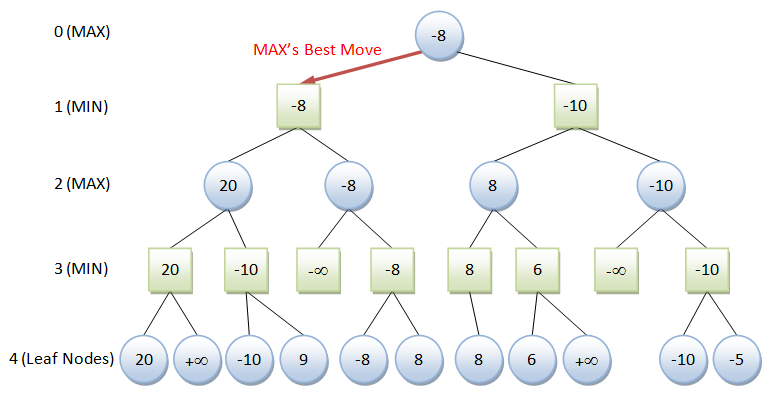
\includegraphics[width=\textwidth]{minimax.png}
\end{figure}

Thuật toán minimax có độ phức tạp lũy thừa theo độ sâu và số lượng nhánh của mỗi node. Do đó nó không khả thi khi áp dụng vào thực tế. 
Tuy nhiên, hiệu năng của thuật toán có thể tăng lên đáng kể nhờ sử dụng cắt tỉa Alpha-Beta. 

\subsection{Thuật toán cắt tỉa Alpha-Beta}
Là thuật toán tìm kiếm cải tiến thuật toán tìm kiếm minimax bằng cách giảm số node phải đánh giá. 
Nó sẽ dừng hoàn toàn đánh giá một nước đi nếu như nó có thể chứng minh được rằng nước đi đó là tồi hơn những nước đi đã được xét. 

Ý tưởng của thuật toán là duy trì 2 giá trị: alpha và beta.
Trong đó alpha đại diện cho giá trị nhỏ nhất của người chơi max được bảo đảm sẽ đạt được và beta đại diện cho giá trị lớn nhất của người chơi min được bảo đảm sẽ đạt được. 
Nếu như giá trị lớn nhất của người chơi min (beta) được bảo đảm đạt được nhỏ hơn giá trị 
nhỏ nhất của người chơi max (alpha) được bảo đảm đạt được (beta <= alpha) thì người chơi max 
sẽ không cần xét đến những node con cháu của node hiện tại đang xét - tương tự với người chơi min. 

\begin{figure}[H]
\caption{Cắt tỉa Alpha-Beta}
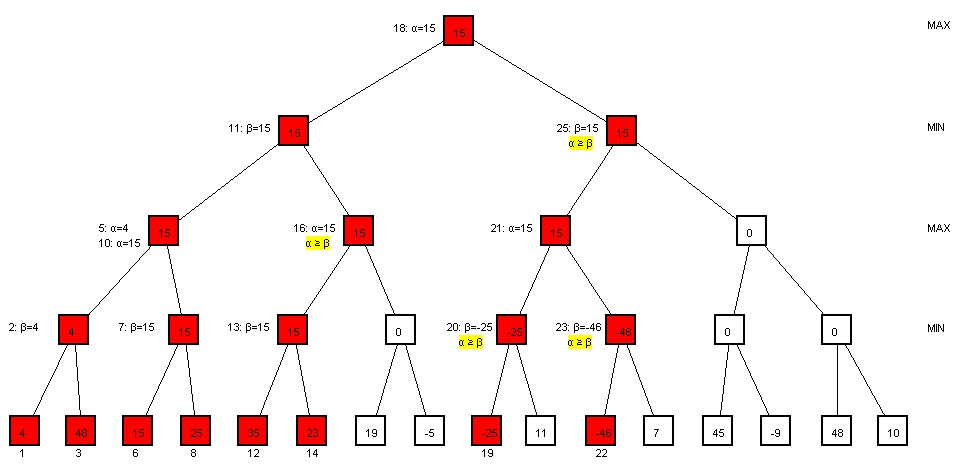
\includegraphics[width=\textwidth]{alpha-beta.jpg}
\end{figure}

Lợi ích của thuật toán thuật toán cắt tỉa Alpha-Beta dựa vào việc các nhánh tìm kiếm trong thuật toán minimax có thể được 
loại bỏ. Từ đó, thời gian tìm kiếm có thể được dành cho những nhánh con ``hứa hẹn'' hơn. Với độ phức tạp thuật toán: 
\begin{itemize}
    \item Trong trường hợp tồi nhất: $O(b^d)$
    \item Trong trường hợp tốt nhất: $O(\sqrt{b^d})$
\end{itemize}
Trong đó $b$ là số lượng node con của một node và $d$ là độ sâu tìm kiếm. \\[0.5cm]

\noindent
Mã giả của thuật toán: \\
\textbf{Input}:
\begin{itemize}
    \item node: Một object của lớp biểu diễn trạng thái của game. 
    \item depth: Độ sâu sẽ tìm kiếm. 
    \item alpha: Giá trị alpha. 
    \item beta: Giá trị beta. 
    \item maximizing: Biến boolen xác định xem là người chơi max (True) hay min (False). 
\end{itemize}
\textbf{Output}: Giá trị heurisic nhỏ nhất / lớn nhất. \\[0.5cm]
\begin{python}
def alphabeta(node, depth, alpha, beta, maximizing):
    if depth == 0 or node.is_terminal():
        return node.heuristic_value()

    if maximizing:
        v = -infinity
        for child in node.children():
            res = alphabeta(child, depth-1, alpha, beta, False)
            v = max(v, res)
            alpha = max(alpha, v)
            if beta <= alpha: 
                break 
        return v
    else:
        v = +infinity
        for child in node.children():
            res = alphabeta(child, depth-1, alpha, beta, True)
            v = min(v, res)
            beta = min(beta, v)
            if beta <= alpha:
                break
        return v
\end{python}

\section{Các thuật toán áp dụng trong game cờ caro}
Mô hình bàn cờ được áp dụng là sử dụng ma trận có kích thước lớn tùy ý. 

\subsection{Xác định các nước đi cho phép}
Ý tưởng: Các nước đi cho phép ở một trạng thái bất kì của game được xác định là khoảng cách tối đa 
là 2 đến ít nhất một quân cờ đã đánh trước đó trong game 
(Quân cờ đầu tiên chỉ có 1 nước có thể đi duy nhất là tại trung tâm bàn cờ). 
\begin{figure}[H]
\centering
\caption{Các nước đi cho phép}
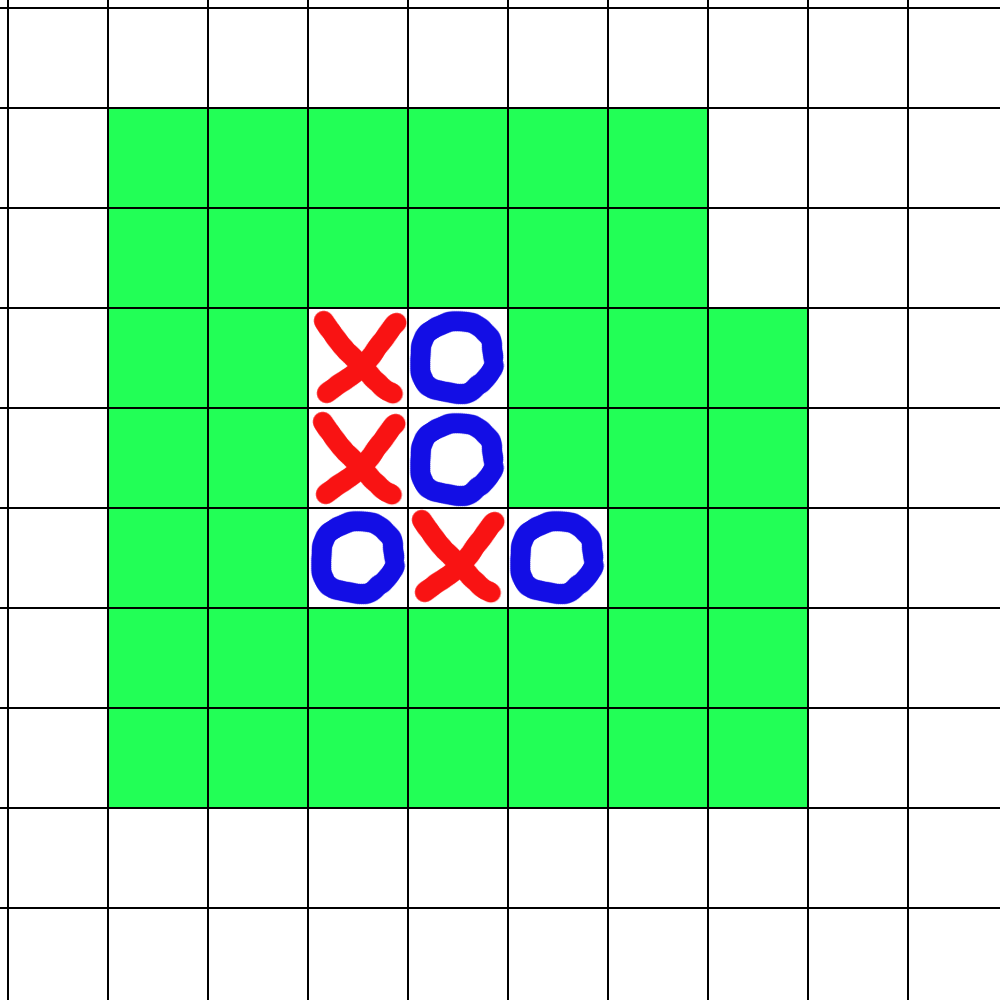
\includegraphics[width=12cm]{legal-actions.png}
\end{figure}

\noindent Cách xác định: Sử dụng một ma trận khác lưu các giá trị số với giá trị ban đầu là 0. 
Với mối ví trị được đánh, 5x5 các ô xung quanh (tính cả tâm) được tăng giá trị lên 1. 
Ban đầu chỉ có vị trí trung tâm là được khởi tạo bằng 1. 
Tất cả những ô mà có số khác 0 và không phải là vị trí đã được đánh, 
thì nó là vị trí cho phép được đánh ở lượt chơi kế tiếp. 

\begin{figure}[H]
\centering
\caption{Xác định các nước đi cho phép}
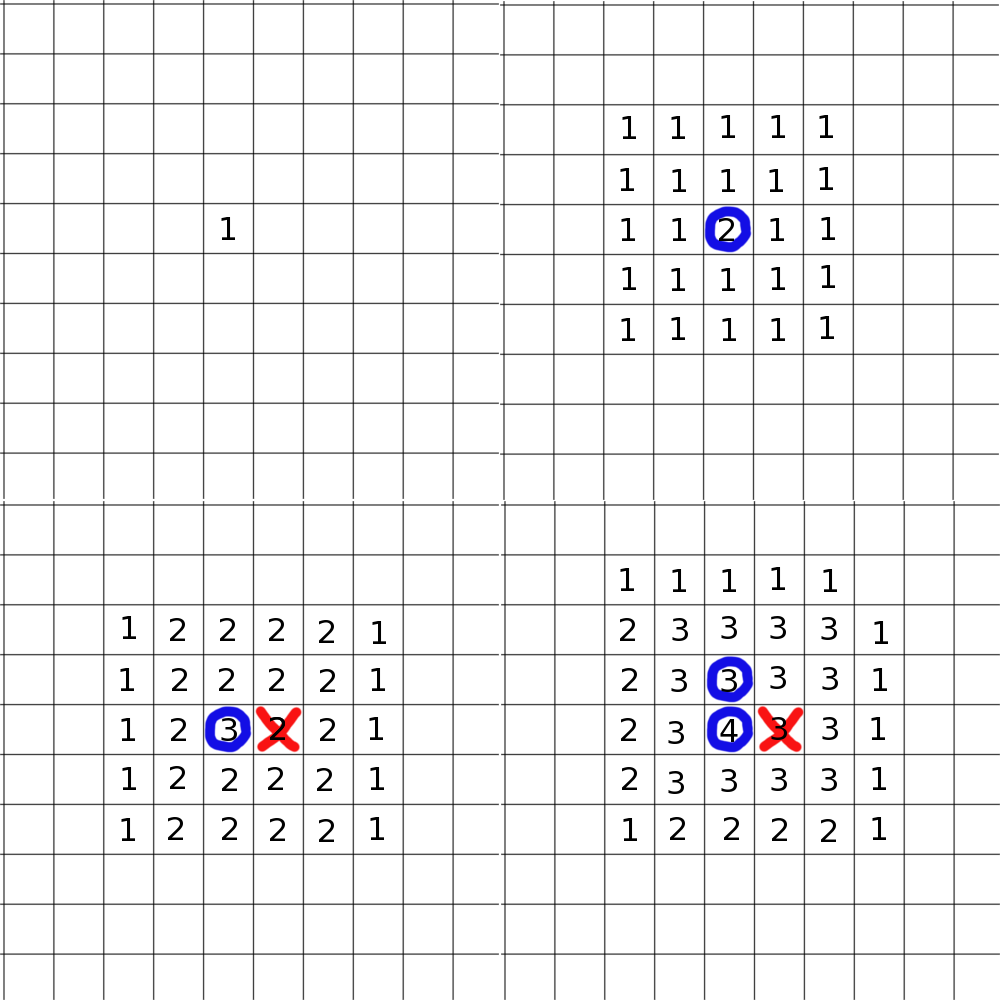
\includegraphics[width=\textwidth]{legal-action-impl.png}
\end{figure}

\subsection{Hàm tính giá trị heuristic}

Từ ma trận các nước đã đi, ta trích ra tất cả những đường (thẳng, ngang hoặc chéo). \\
Ví dụ đường chéo: 
\begin{figure}[H]
\centering
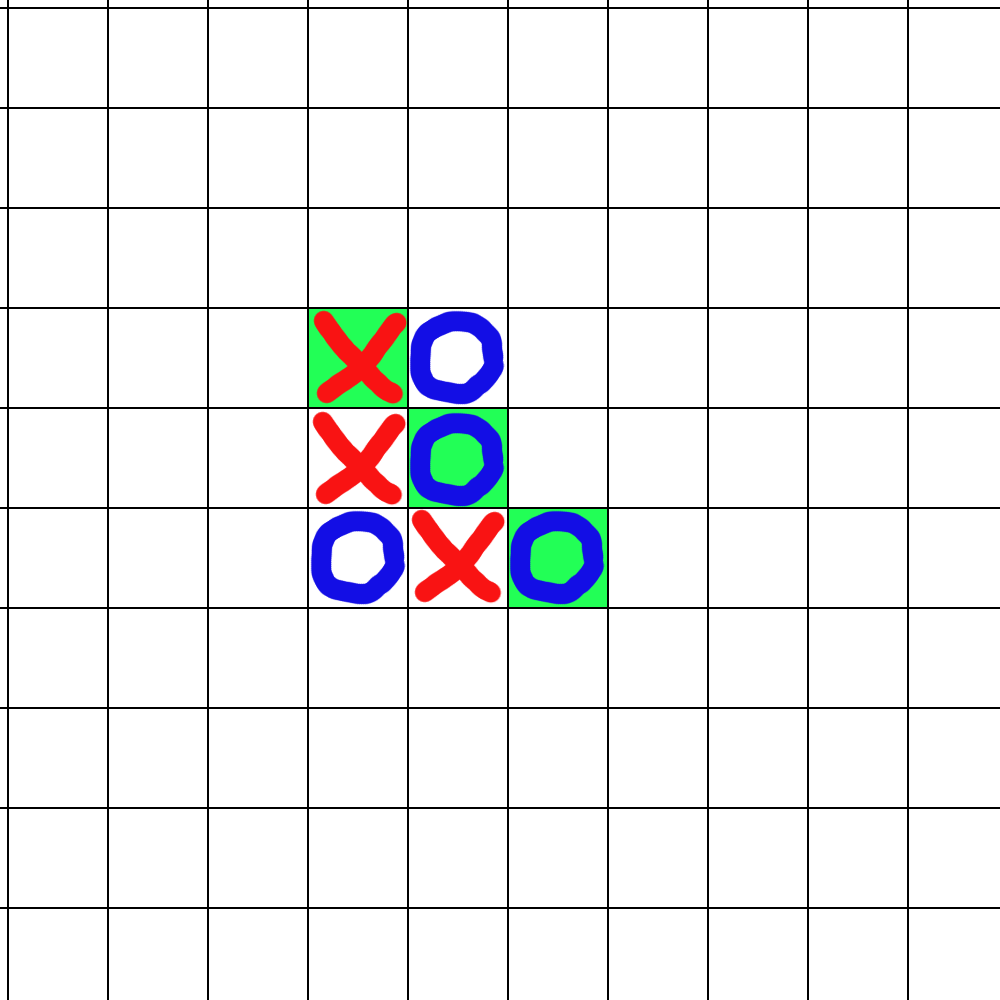
\includegraphics[width=8cm]{matrix-line.png}
\end{figure}
\noindent Sẽ được trích thành một vector: 
\begin{figure}[H]
\centering

\includegraphics[width=4cm]{line.png}
\end{figure}

Từ các đường đã trích ra, ta sẽ tính điểm số trên các đường này rồi cộng tổng các điếm sổ lại. 
Các đường sau đó được trích ra thành các đoạn để có thể dễ dàng tính trọng số. 
Việc trích thành các đoạn ra sao cũng phụ thuộc vào người chơi (quân X hay O) đang được xét. \\
Ví dụ đường: 
\begin{figure}[H]
\centering

\includegraphics[width=8cm]{line2.png}
\end{figure}
\noindent Sẽ được trích thành 2 đoạn (nếu được xét theo X): 
\begin{figure}[H]
\centering

\includegraphics[width=5cm]{segment1.png}
\end{figure}
\begin{figure}[H]
\centering

\includegraphics[width=4cm]{segment2.png}
\end{figure}
Ta sẽ tính điểm dựa trên từng đoạn, cộng tổng sẽ được điểm của một đường. 
Từ đó ta tính được giá trị heuristic của một trạng thái trong game. 


\end{document}
